% multiple1902 <multiple1902@gmail.com>
% intro.tex
% Copyright 2011~2012, multiple1902 (Weisi Dai)
% https://code.google.com/p/xjtuthesis/
%
% It is strongly recommended that you read documentations located at
%   http://code.google.com/p/xjtuthesis/wiki/Landing?tm=6
% in advance of your compilation if you have not read them before.
%
% This work may be distributed and/or modified under the
% conditions of the LaTeX Project Public License, either version 1.3
% of this license or (at your option) any later version.
% The latest version of this license is in
%   http://www.latex-project.org/lppl.txt
% and version 1.3 or later is part of all distributions of LaTeX
% version 2005/12/01 or later.
%
% This work has the LPPL maintenance status `maintained'.
%
% The Current Maintainer of this work is Weisi Dai.
%

\chapter{论文相关理论与技术}
\echapter{Relative Theory and Technology}

    文字检测按照其研究目标和存储介质的不同,可分为数字图像文字检测、视频图像中的文字检测和自然场景图像中的文字检测。其中,由于自然场景中的文字会遭受背景复杂多样性,以及图像质量易被光照、阴影、遮挡等环境因素影响,致使自然场景图像的文字检测相比于其它图像对检测算法的健壮性要求更高。这些年来,学者们在文字检测领域进行了大量的研究和实验工作,提出了许多不同的方法,检测效果也在逐年提升。但是在ICDAR等公开数据集上的测试结果表明,目前的这些自然场景图像中的文字检测结果仍有提高空间,所以仍是文字检测领域内的一个热点方向。场景图像文字检测方法根据流程不同,可分为基于区域、连通部件以及边缘三类方法。下面整理并分别介绍近年来这三类文字检测的相关方法。

    \section{基于区域的场景文字检测方法}
    \esection{Region-based Method}

    基于区域的文字检测方法,是基于文子有别于背景的视觉特征来区分文字区域与背景区域的。使用较多的视觉特征主要包括纹理、边缘及颜色等。因为每个文字都是用来传递信息的特定符号,其纹理与一般背景并不相同,同时文字相比于背景也有着更强的对比度和显著的颜色,所以包含着文字的那些区域和背景图像区域有着不同的视觉特征,因而可以用来区分文字区域与非文字区域。

    \begin{figure}[!h]
    \centering
    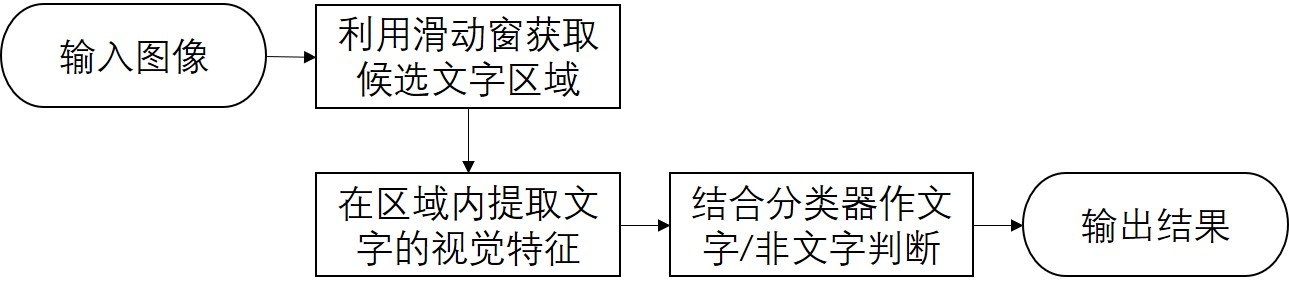
\includegraphics[width=\textwidth]{c2_region_based.jpg}
    \caption{基于区域的文字检测方法的流程示例}
    \label{fig.c2_region_based}
    \end{figure}

    大部分基于区域的方法一般都会利用滑动窗来获取候选的包含文字的局部图像区域,因此在有些方法中也称其为基于滑动窗的文字检测算法。如图\ref{fig.c2_region_based} 所示,这是1个典型的基于区域的文字检测方法的流程示例。在该流程示例中,首先利用滑动窗来得到局部图像区域以作为候选区域,然后提取区域中的颜色、纹理等视觉特征,最后结合分类器以进行文字与非文字区域的分类判别,输出结果是检测出来的文字区域。

    Chen等\cite{Chen2004Detecting}利用滑动窗扫描得到文字区域并获取区域中的79个特征,然后构造4个级联的Adaboost 分类器来分类和筛选这些候选文字区域,最后用OCR软件识别图像中文字信息。其中4个级联的分类器是由不同的文字底层特征构造而成的弱分类器,通过利用Adaboost方法将这些弱分类器组合学习而获得1个分类文字与背景的强分类器。用于训练弱分类器的三组特征分别是:候选区域内竖直和水平方向灰度的标准差与平均值;区域内的统计梯度信息;区域内边缘组合特征。而本方法中使用的79个特征,分散在4层的级联分类器中,分别有1、10、30和50维文字特征。最后OCR使用的技术是用Niblack方法来二值化检测到的文字区域以识别出图像中的文字。

    \begin{table*}[!h]
    \centering
    \caption{基于区域的相关文字检测方法}
    \begin{tabular}{p{0.17\textwidth}|p{0.1\textwidth}| p{0.63\textwidth}}
    \hline
    作者 & 年份 & 方法概述 \\
    \hline
    Chen等\cite{Chen2004Detecting} & 2004年 & 区域特征,滑动窗检测,以及SVM分类器;\\
    Pan等\cite{Pan2011A} & 2011年 &   条件随机场,滑动窗检测,以及waldBoost分类器\\
    Wang等\cite{Wang2012End} & 2012年 & 卷积神经网络和滑动窗检测 \\
    Zhang等\cite{Zhang2015Symmetry} & 2015年 & 对称性特征,滑动窗检测以及卷积神经网络 \\
    \hline
    \end{tabular}
    \label{tab.c2_region_based}
    \end{table*}

    \section{基于连通部件的场景文字检测方法}
    \esection{Connected Component-based Method}

    \begin{table*}[!h]
    \centering
    \caption{基于连通部件的相关文字检测方法}
    \begin{tabular}{p{0.17\textwidth}|p{0.1\textwidth}| p{0.63\textwidth}}
    \hline
    作者 & 年份 & 方法概述 \\
    \hline
    Epshetein等\cite{Epshtein2010Detecting} & 2010年 & 候选文字筛选,笔画宽度转换SWT,文本行生成;\\
    Neumann等\cite{Neumann2011Text} & 2011年 &   最稳定极值区域MSER,穷举搜索\\
    Dollar等\cite{Dollar2015Fast} & 2015年 & 结构化边缘检测子,随机森林分类器 \\
    Yu等\cite{Yu2016Scene} & 2016年 & 文字的特征池,文字的边缘重组,以及SVM分类器 \\
    \hline
    \end{tabular}
    \label{tab.c2_connected_component_based}
    \end{table*}

    \section{本章小结}
    \esection{Brief Summary}

